\documentclass{ximera}

\graphicspath{{./}{thePythagoreanTheorem/}{deMoivreSavesTheDay/}{complexNumbersFromDifferentAngles/}}

\usepackage{tikz}
\usepackage{tkz-euclide}
\usetkzobj{all}
\tikzstyle geometryDiagrams=[ultra thick,color=blue!50!black]
\newcommand{\tri}{\triangle}
\renewcommand{\l}{\ell}
\renewcommand{\P}{\mathcal{P}}
\newcommand{\R}{\mathbb{R}}
\newcommand{\Q}{\mathbb{Q}}

\newcommand{\Z}{\mathbb Z}

\renewcommand{\vec}{\mathbf}
\renewcommand{\d}{\,d}



%% Egyptian symbols

\usepackage{multido}
\newcommand{\egmil}[1]{\multido{\i=1+1}{#1}{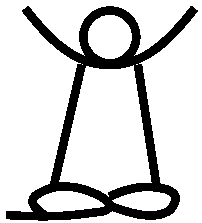
\includegraphics[scale=.1]{egyptian/egypt_person.pdf}\hspace{0.5mm}}}
\newcommand{\eghuntho}[1]{\multido{\i=1+1}{#1}{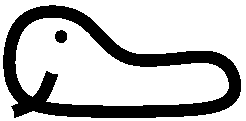
\includegraphics[scale=.1]{egyptian/egypt_fish.pdf}\hspace{0.5mm}}}
\newcommand{\egtentho}[1]{\multido{\i=1+1}{#1}{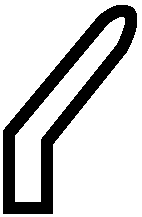
\includegraphics[scale=.1]{egyptian/egypt_finger.pdf}\hspace{0.5mm}}}
\newcommand{\egtho}[1]{\multido{\i=1+1}{#1}{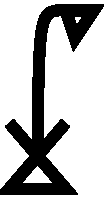
\includegraphics[scale=.1]{egyptian/egypt_lotus.pdf}\hspace{0.5mm}}}
\newcommand{\eghun}[1]{\multido{\i=1+1}{#1}{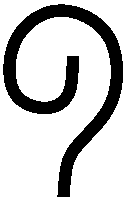
\includegraphics[scale=.1]{egyptian/egypt_scroll.pdf}\hspace{0.5mm}}}
\newcommand{\egten}[1]{\multido{\i=1+1}{#1}{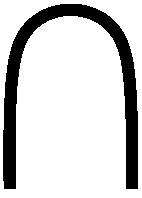
\includegraphics[scale=.1]{egyptian/egypt_heel.pdf}\hspace{0.5mm}}}
\newcommand{\egone}[1]{\multido{\i=1+1}{#1}{
\includegraphics[scale=.1]{egyptian/egypt_stroke.pdf}\hspace{0.5mm}}}
\newcommand{\egyptify}[7]{
 \multido{\i=1+1}{#1}{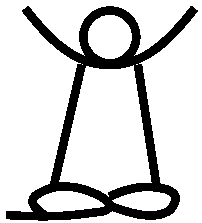
\includegraphics[scale=.1]{egyptian/egypt_person.pdf}\hspace{0.5mm}}
 \multido{\i=1+1}{#2}{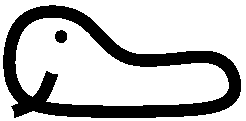
\includegraphics[scale=.1]{egyptian/egypt_fish.pdf}\hspace{0.5mm}}
 \multido{\i=1+1}{#3}{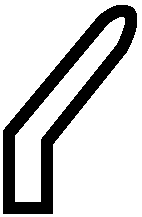
\includegraphics[scale=.1]{egyptian/egypt_finger.pdf}\hspace{0.5mm}}
 \multido{\i=1+1}{#4}{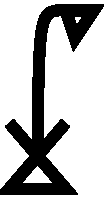
\includegraphics[scale=.1]{egyptian/egypt_lotus.pdf}\hspace{0.5mm}}
 \multido{\i=1+1}{#5}{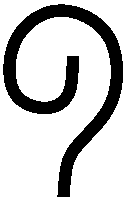
\includegraphics[scale=.1]{egyptian/egypt_scroll.pdf}\hspace{0.5mm}}
 \multido{\i=1+1}{#6}{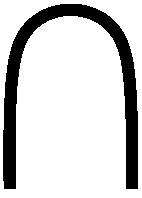
\includegraphics[scale=.1]{egyptian/egypt_heel.pdf}\hspace{0.5mm}}
 \multido{\i=1+1}{#7}{
\includegraphics[scale=.1]{egyptian/egypt_stroke.pdf}\hspace{0.5mm}}
 \hspace{.5mm}
}




\title{Triangles on a Cone}	
\begin{document}
\begin{abstract}
In this activity we investigate the sum of the interior angles of a triangle.
\end{abstract}
\maketitle


\subsection*{Euclidean geometry}

We are going to investigate why the interior angles of a triangle sum
to $180^\circ$. We won't be alone on this journey; we'll have help.
Meet Louie Llama:\index{Louie Llama}
\begin{image}
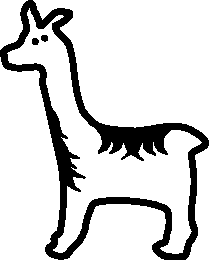
\includegraphics[height=1in]{llama.pdf}
\end{image}

Louie Llama is rather radical for a llama and doesn't mind being
rotated.

\begin{question} 
Draw a picture of Louie Llama rotated $90^\circ$ counterclockwise.
\end{question}

\begin{question} 
Draw a picture of Louie Llama rotated $180^\circ$ counterclockwise.
\end{question}

\begin{question} 
Draw a picture of Louie Llama rotated $360^\circ$ counterclockwise.
\end{question}

\begin{question} Sometimes Louie Llama likes to walk around lines he finds:
\begin{image}
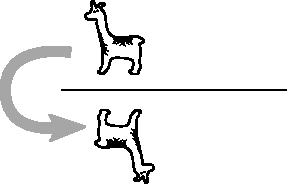
\includegraphics{llamaLines.pdf}
\end{image}
Through what angle did Louie Llama just rotate?
\end{question}


Now we're going to watch Louie Llama go for a walk. Draw yourself any
triangle.  Actually, draw a crazy scalene triangle---those are the kind that Louie
Llama likes best. Louie Llama is going to proudly parade around this
triangle. When Louie Llama walks around corners he rotates. Check
it out:
\begin{image}
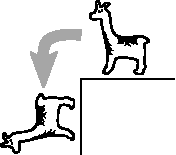
\includegraphics{llamaCorner.pdf}
\end{image}
Take your triangle and denote the measure of its angles as $a$, $b$,
and $c$. Start Louie Llama out along a side adjacent to the angle of
measure $a$. He should be on the outside of the triangle, his feet
should be pointing toward the triangle, and his face should be
pointing toward the angle of measure $b$.
\begin{question} 
Sketch Louie Llama walking to the angle of measure $b$. Walk him
around the angle. As he goes around the angle his feet should always
be pointing toward the triangle. Through what angle did Louie Llama
just rotate?
\end{question}

\begin{question}
Sketch Louie Llama walking to the angle of measure $c$. Walk him
around the angle. Through what angle did Louie Llama just rotate?
\end{question}

\begin{question}
Finally, sketch Louie Llama walking back to the angle of measure
$a$. Walk him around the angle. He should be back at his starting
point. Through what angle did Louie Llama just rotate?
\end{question}

\begin{question} 
All in all, how many degrees did Louie Llama rotate in his walk?
\end{question}

\begin{question} 
Write an equation where the right-hand side is Louie Llama's total
rotation and the left-hand side is the sum of each rotation around the
angle. Can you solve for $a+b+c$?
\end{question}



\subsection*{A noneuclidean geometry}


Put a dot at the center of a blank sheet of paper and call it $O$.
Use a protractor to draw an angle of $50^\circ$ with vertex at the
point $O$ and sides extending all the way out to the edge of the
paper.  Cut the paper along one side of the angle and one side only.
Make a cone by moving the cut edge to the other side of the angle you
drew.  This cone (extended infinitely) is your universe.


\begin{question}
Make a triangle in your universe that surrounds $O$. To do this,
unfold your universe and lay it out flat on the desk and make the
sides with your ruler.  When a side gets to the cut side of your
angle, put the other side of the angle on top and keep going.
\end{question}

\begin{question}
You measure angles on your universe by laying the paper out flat and
measuring the angles on the paper. Measure the angles in your
triangle, what do they sum to?
\end{question}


\begin{question}
Repeat the questionlems above, but this time cut an angle of $40^\circ$ to
make your cone. What do you notice?
\end{question}

Let's see if we can explain this. Do you know who is eager to help
you? That's right: Louie Llama.
\begin{image}
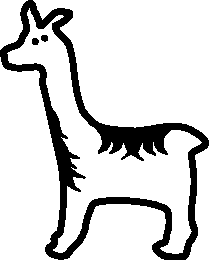
\includegraphics[height=1in]{llama.pdf}
\end{image}

\begin{question}
Take your triangle and denote the measure of its angles as $a$, $b$,
and $c$. We would like to parade Louie around the triangle. There is
only one catch: What happens to Louie when he passes over the ``cut?''
Draw some pictures and see if you can figure it out.
\end{question}

Start Louie Llama out along a side adjacent to the angle of measure
$a$. He should be on the outside of the triangle, his feet should be
pointing toward the triangle, and his face should be pointing toward
the angle of measure $b$. Continue this process and walk him all
around the triangle. When he gets to the ``cut'' put the paper
together, and let him continue his walk.

\begin{question} 
Through what angle does Louie rotate when he strolls around a vertex?
\end{question}

\begin{question}
How many degrees did the ``cut'' rotate Louie? 
\end{question}

\begin{question} 
All in all, how many degrees did Louie Llama rotate in his walk?
\end{question}


\begin{question}
If a cone is made on a sheet of paper with a cut of $\theta$ degrees,
and a triangle is made surrounding the point of the cone, what is the
sum of the degrees of this triangle?
\end{question}




\begin{question}
Explain why not all of Euclid's postulates could hold in this
universe. Exactly which postulates don't hold?
\end{question}
\end{document}
